% CVPR 2025 Paper Template; see https://github.com/cvpr-org/author-kit

\documentclass[10pt,twocolumn,letterpaper]{article}

%%%%%%%%% PAPER TYPE  - PLEASE UPDATE FOR FINAL VERSION
\usepackage{cvpr}              % To produce the CAMERA-READY version
% \usepackage[review]{cvpr}      % To produce the REVIEW version
% \usepackage[pagenumbers]{cvpr} % To force page numbers, e.g. for an arXiv version

% Import additional packages in the preamble file, before hyperref
%
% --- inline annotations
%
\newcommand{\red}[1]{{\color{red}#1}}
\newcommand{\todo}[1]{{\color{red}#1}}
\newcommand{\TODO}[1]{\textbf{\color{red}[TODO: #1]}}
% --- disable by uncommenting  
% \renewcommand{\TODO}[1]{}
% \renewcommand{\todo}[1]{#1}



% It is strongly recommended to use hyperref, especially for the review version.
% hyperref with option pagebackref eases the reviewers' job.
% Please disable hyperref *only* if you encounter grave issues, 
% e.g. with the file validation for the camera-ready version.
%
% If you comment hyperref and then uncomment it, you should delete *.aux before re-running LaTeX.
% (Or just hit 'q' on the first LaTeX run, let it finish, and you should be clear).
\definecolor{cvprblue}{rgb}{0.21,0.49,0.74}
\usepackage[pagebackref,breaklinks,colorlinks,allcolors=cvprblue]{hyperref}
\usepackage{subcaption}
\usepackage{amsmath}
\usepackage{graphicx} % Include this in the preamble
% \usepackage[noend]{algpseudocode}
% \usepackage[ruled,vlined]{algorithm2e}

\usepackage{multirow}
\usepackage{vector}
\usepackage{booktabs}
\usepackage{pgfplots}
\pgfplotsset{compat=1.18}
\usepackage{siunitx}
% \usepackage{ctable}
\usepackage{algorithm}
% \usepackage{algorithmic}
\usepackage[noend]{algcompatible}
\usepackage{hyperref} 


\renewcommand\algorithmicthen{}
\renewcommand\algorithmicdo{}



\usetikzlibrary{arrows}
\usetikzlibrary{angles}


%%%%%%%%% PAPER ID  - PLEASE UPDATE
\def\paperID{*****} % *** Enter the Paper ID here
\def\confName{CVPR}
\def\confYear{2025}

%%%%%%%%% TITLE - PLEASE UPDATE
\title{Beyond Gradient Averaging in Parallel Optimization:\\ Improved Robustness through Gradient Agreement Filtering}

%%%%%%%%% AUTHORS - PLEASE UPDATE
\author{Francois Chaubard\\
{\tt\small fchaubar@stanford.edu}
% For a paper whose authors are all at the same institution,
% omit the following lines up until the closing ``}''.
% Additional authors and addresses can be added with ``\and'',
% just like the second author.
% To save space, use either the email address or home page, not both
\and
Duncan Eddy\\
{\tt\small deddy@stanford.edu} \\
Stanford University\\
% 496 Lomita Mall\\
% Stanford, CA 94305\\
\and
Mykel J. Kochenderfer\\
{\tt\small mykel@stanford.edu}
}

\begin{document}
\maketitle
\begin{abstract}
Diffusion Models have emerged as powerful generative models for high-quality image synthesis, with many subsequent image editing techniques based on them. However, the ease of text-based image editing introduces significant risks, such as malicious editing for scams or intellectual property infringement. Previous works have attempted to safeguard images from diffusion-based editing by adding imperceptible perturbations. These methods are costly and specifically target prevalent Latent Diffusion Models (LDMs), while Pixel-domain Diffusion Models (PDMs) remain largely unexplored and robust against such attacks. Our work addresses this gap by proposing a novel attacking framework with a feature representation attack loss that exploits vulnerabilities in denoising UNets and a latent optimization strategy to enhance the naturalness of protected images. Extensive experiments demonstrate the effectiveness of our approach in attacking dominant PDM-based editing methods (e.g., SDEdit) while maintaining reasonable protection fidelity and robustness against common defense methods. Additionally, our framework is extensible to LDMs, achieving comparable performance to existing approaches.
\end{abstract}
    
\section{Introduction}
\label{sec:intro}

\begin{figure*}[t]
\centering
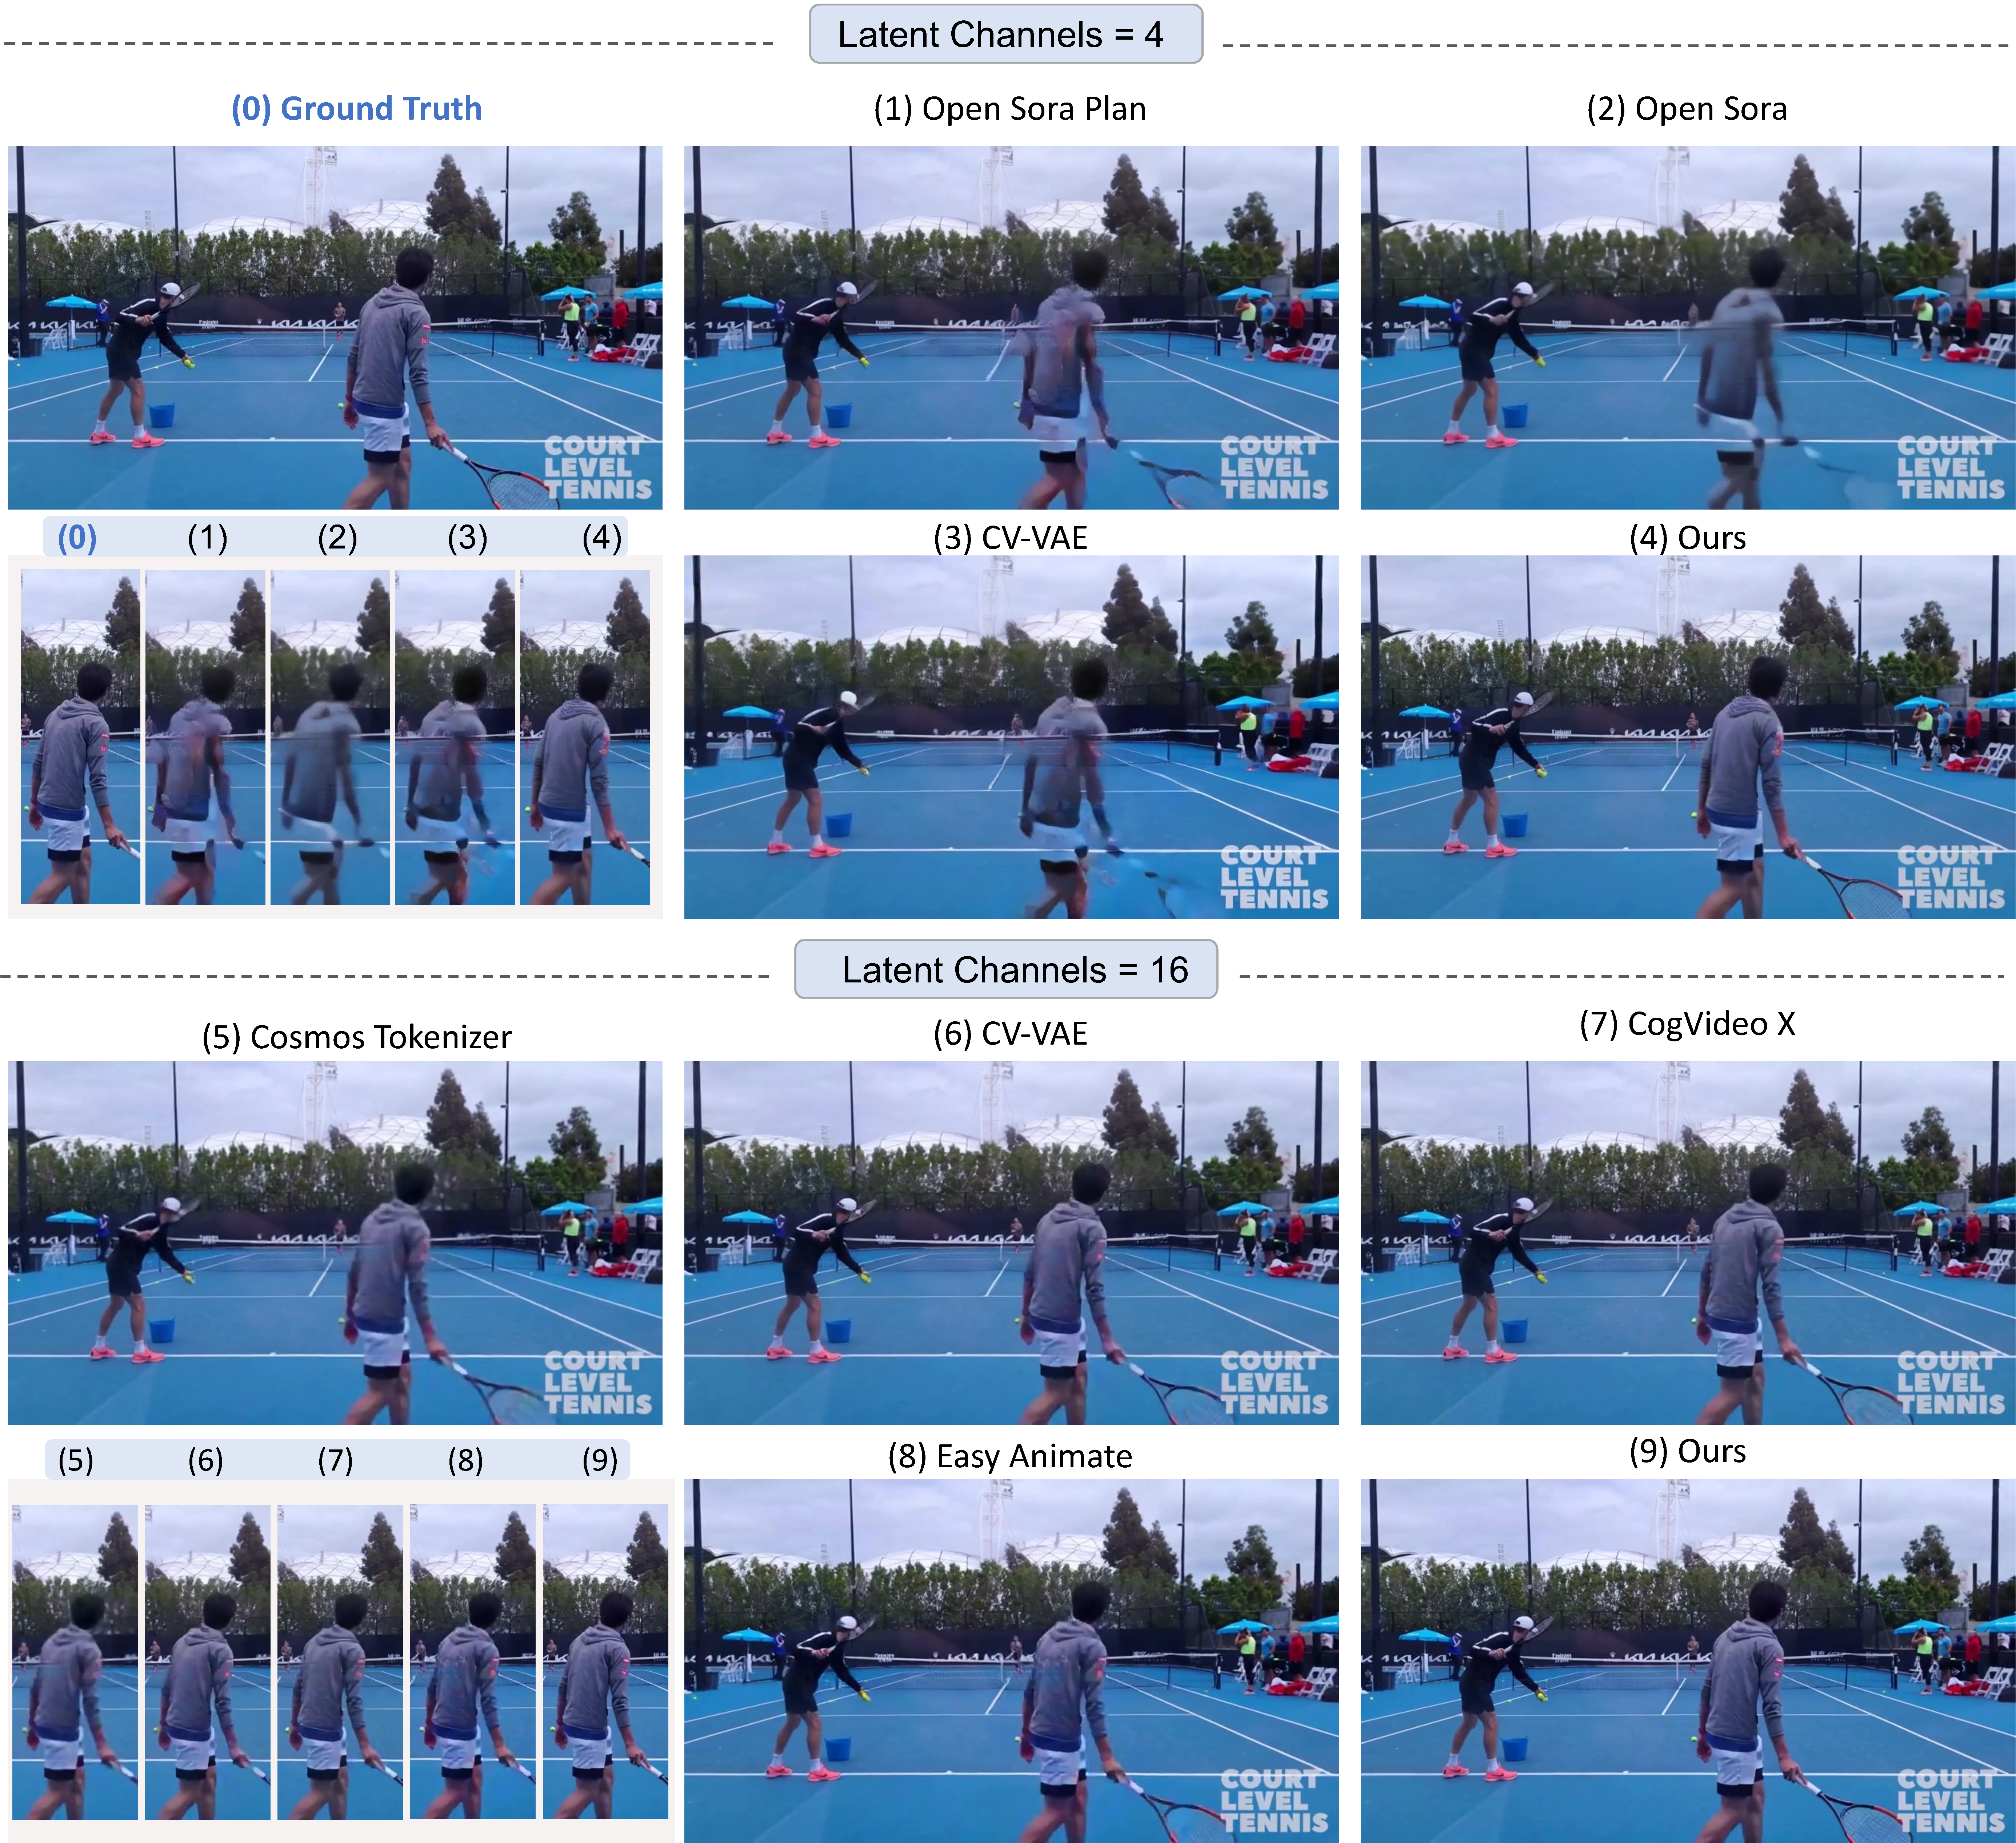
\includegraphics[width=1.0\textwidth]{images/fig1-4and16.pdf}
\caption{
Our reconstruction results compared with a line of three recent strong baseline approaches. 
The ground truth frame is (0). Our model significantly outperforms previous methods, especially under large motion scenarios such as people doing sports.
}
\label{fig:teaser}
\vspace{-3mm}
\end{figure*}



Given the significant attention in the field of video generation, Latent Video Diffusion Models (LVDMs)~\cite{blattmann2023stable, blattmann2023align, he-lvdm, zhou2022magicvideo, he-videocrafter1} have emerged as a popular framework. They have been successfully applied to powerful text-to-video models such as Sora~\cite{videoworldsimulators2024}, VideoCrafter~\cite{he-videocrafter1, chen2024videocrafter2overcomingdatalimitations}, and CogVideoX~\cite{yang2024cogvideox}.
Different from directly generating video pixels, LVDMs generate latent video representations in a compact latent space. This is achieved by first training a Video VAE to encode videos into this latent space.
%
Thus, Video VAE, as a key and fundamental component of LVDMs, has attracted great attention recently.
%
An effective Video VAE can help to reduce the training costs of video diffusion models while improving the final quality of the generated videos.
%
Initially, a series of studies adopt the image VAE from Stable Diffusion~\cite{rombach2022high} for video generation tasks, including AnimateDiff~\cite{guoanimatediff}, MagicVideo~\cite{zhou2022magicvideo}, VideoCrafter1~\cite{he-videocrafter1}, and VideoCrafter2~\cite{chen2024videocrafter2overcomingdatalimitations}. 
%
However, directly adopting an image VAE and compressing video on a frame-by-frame basis leads to temporal flickering due to the lack of temporal correlation. Additionally, the information redundancy along the temporal dimension is not reduced, leading to low training efficiency for subsequent latent video diffusion models.
%
From the introduction of Sora, which compresses videos both temporally and spatially through a Video VAE, a series of studies have emerged that aim to replicate Sora and train their own Video VAEs, including Open Sora~\cite{opensora}, Open Sora Plan~\cite{pku_yuan_lab_and_tuzhan_ai_etc_2024_10948109}, CV-VAE~\cite{zhao2024cv}, CogVideoX~\cite{yang2024cogvideox}, EasyAnimate~\cite{xu2024easyanimatehighperformancelongvideo}, and Cosmos Tokenizer~\cite{cosmos_token}.
%
However, the performance of the current video VAE suffers from many problems, including motion ghost, low-level temporal flickering, blurring (faces, hands, edges, texts), and motion stuttering (lack of correct temporal transition).
% as shown in Fig.~\ref{fig:teaser}.


In this work, we propose a novel cross-modal Video VAE with better spatial and temporal modeling ability in order to solve the aforementioned challenge problems and obtain a robust and high-quality Video VAE.
%
First, we examine different designs for spatial and temporal compression, including simultaneous spatial-temporal (ST) compression and sequential ST compression. 
%
We observed that simultaneous ST compression achieves better low-level temporal smoothness and texture stability, while sequential ST compression achieves better motion recovery, particularly in scenarios of large motion.
%
Thus, we propose a novel architecture that integrates the advantages of both methods and enables effective video detail and motion reconstruction.

Second, we observed that the normally used datasets for text-to-video generation contain text-video pairs. 
Also, during decoding, a text description exists as it serves as the input in the first stage, \textit{i.e.}, the video latent generation stage.
%
To this end, we integrate the text information into the encoding and decoding procedure and propose the first Cross-modal Video VAE.
%
We carefully study how text guidance can be integrated into the spatiotemporal backbone and the mechanism of spatial and temporal semantic guidance. 

In addition, our cross-modal video VAE supports image-video joint training.
To achieve this, we design our network with a fully spatiotemporal factorized architecture, and we feed image and video batches alternately to the network. 
%
During image batches, the data only forwards the spatial part of the network, with the temporal modules being skipped. During video batches, the video forwards both spatial and temporal modules. We also demonstrate that image joint training is crucial for training a video VAE.
%
In summary, our contributions are as follows:
\begin{itemize}
    \item We propose an effective and robust Video VAE, conduct extensive experiments, and achieve the state-of-the-art.
    \item We propose an optimal spatiotemporal modeling approach for Video VAE.
    \item We propose the first cross-modal video VAE that leverages the information from other modalities, i.e., text descriptions, to the best of our knowledge.
    \item Our video VAE is designed and trained to be versatile to conduct both image and video compression. 
\end{itemize}


\section{Methods}
\label{sec:methods}

We consider the problem of how to most efficiently estimate an accurate gradient by aggregating micro-gradients during distributed training while preventing memorization and minimizing the compute budget. The core algorithm is presented in \Cref{alg:gaf}. Consider a training set $\mathcal{N}$ of size $n$. In traditional SGD, an update to the model parameters $\theta$ is computed by sampling a minibatch $\mathcal{B} \subset \mathcal{N}$ of size $|\mathcal{B}| = b$, calculating the gradient $\nabla_\theta \mathcal{L}(\mathcal{B}; \theta)$, and applying the following update rule
\begin{equation} \label{eq:sgd_update}
    \theta \leftarrow \theta - \eta \nabla_\theta \mathcal{L}(\mathcal{B}; \theta)
\end{equation}
where $\eta$ is the learning rate, and $\mathcal{L}(\mathcal{B}; \theta)$ is the loss function over the minibatch $\mathcal{B}$.

Due to GPU memory constraints, training is parallelized across multiple GPUs by computing the gradient for a \textit{macrobatch} of data comprised of multiple \textit{microbatches}. A microbatch $\mathcal{U}_i$ is a subset of samples within a larger macrobatch $\mathcal{M}$ where the microbatch data is small enough to fit in the VRAM of a single GPU. Each microbatch has size $|\mathcal{U}_i| = u$, a macrobatch $\mathcal{M}$ consists of multiple microbatches, i.e., $\mathcal{M} = \{\mathcal{U}_1, \mathcal{U}_2, \dots, \mathcal{U}_k\}$ with $|\mathcal{M}| = m = k \cdot u$. Typically $u \ll m$.

For each microbatch $\mathcal{U}_i$, a micro-gradient $\nabla_\theta \mathcal{L}(\mathcal{U}_i; \theta)$ is computed. The final gradient used to update $\theta$ is obtained by averaging the micro-gradients across all microbatches in $\mathcal{M}$
\begin{equation} \label{eq:macro_batch_eq_without_GAF}
    \nabla_\theta \mathcal{L}(\mathcal{M}; \theta) = \frac{1}{k} \sum_{i=1}^k \nabla_\theta \mathcal{L}(\mathcal{U}_i; \theta).
\end{equation}
The SGD update with the macrobatch gradient is then
\begin{equation} \label{eq:sgd_macrobatch_update}
    \theta \leftarrow \theta - \eta \nabla_\theta \mathcal{L}(\mathcal{M}; \theta).
\end{equation}

\begin{algorithm}[h]
\caption{Gradient Agreement Filtering (GAF)}
\label{alg:gaf}
\begin{algorithmic}[1]
\STATE \textbf{Input:} Training set $\mathcal{N}$, macrobatch size $m$, microbatch size $u$, training GPUs $k$, cosine distance threshold $\tau$, learning rate $\eta$, total training steps $T$
\FOR{$t \in [1, T]$}
    \STATE \textsc{sample} $\mathcal{M}_t \sim \mathcal{N}, \;$ {\upshape{s.t.}} $\; |\mathcal{M}_t| = m$
    \STATE \textsc{distribute} $\mathcal{M}_t $ \upshape{into} $k \; $\upshape{microbatches} $\mathcal{U}_k$
    \STATE \quad $\text{s.t.} \; \bigcup_{i=1}^{k} \mathcal{U}_{i} = \mathcal{M}_t, |\mathcal{U}_{i}| = u, m = u \times k$
    \STATE \textsc{sample} $s \sim \;$ \textsc{categorical}$(1, 2, \dots, k)$
    \STATE $\mathbf{g} \leftarrow \nabla_\theta \mathcal{L}(\mathcal{U}_s; \theta)$
    \STATE $\mathbf{c} \leftarrow 1$
    \FOR{$i \in [1, k], i \neq s$}
        \STATE $\mathbf{g}_i \leftarrow \nabla_\theta \mathcal{L}(\mathcal{U}_i; \theta)$
        % \FOR{$j \in [1, |\mathcal{G}|]$}
        \STATE $D_c(\mathbf{g}_i,\mathbf{g}) \leftarrow 1 - \frac{\mathbf{g}_i^T \mathbf{g}}{\|\mathbf{g}_i\| \|\mathbf{g}\|}$
        \IF{$D_c(\mathbf{g}_i,\mathbf{g}) \leq \tau$}
            \STATE $\mathbf{g} \leftarrow \mathbf{g} + \mathbf{g_i}$
            \STATE $\mathbf{c}   \leftarrow \mathbf{c} + 1$
        \ENDIF
        % \ENDFOR
        \IF{$c > 1$}
            \STATE $\mathbf{g}_{\text{GAF}} \leftarrow \frac{\mathbf{g}}{c}$
            \STATE $\theta \leftarrow \theta - \eta \mathbf{g}_{\text{GAF}}$
        \ELSE
            \STATE \textsc{continue}
        \ENDIF
    \ENDFOR
\ENDFOR
\end{algorithmic}
\end{algorithm}

\subsection{Gradient Agreement Filtering (GAF)}

Gradient agreement filtering is an approach to aggregate micro-gradients that improves upon simply averaging all micro-gradients $\nabla_\theta \mathcal{L}(\mathcal{U}_i; \theta) \; \forall \; \mathcal{U}_i \in \mathcal{M}$. The approach is motivated by the following observation. If we train on completely random data (white noise), a model will overfit the train set but cosine distance will never fall below 0.99 after just a few iterations, as seen in \Cref{fig:random_data_run}. This suggests that we can prevent overfitting on noise by simply skipping updates where the micro-gradients have greater than 0.99 cosine distance. The cosine distance $D_c$ between two vectors $\mathbf{x}$ and $\mathbf{y}$ is
\begin{equation} \label{eq:cdist}
    D_c(\mathbf{x},\mathbf{y}) = 1 - \frac{\mathbf{x}^T\mathbf{y}}{\|\mathbf{x}\|\|\mathbf{y}\|}
\end{equation}

\begin{figure}[th]
    \centering
    \begin{subfigure}{0.975\linewidth}
        \centering
        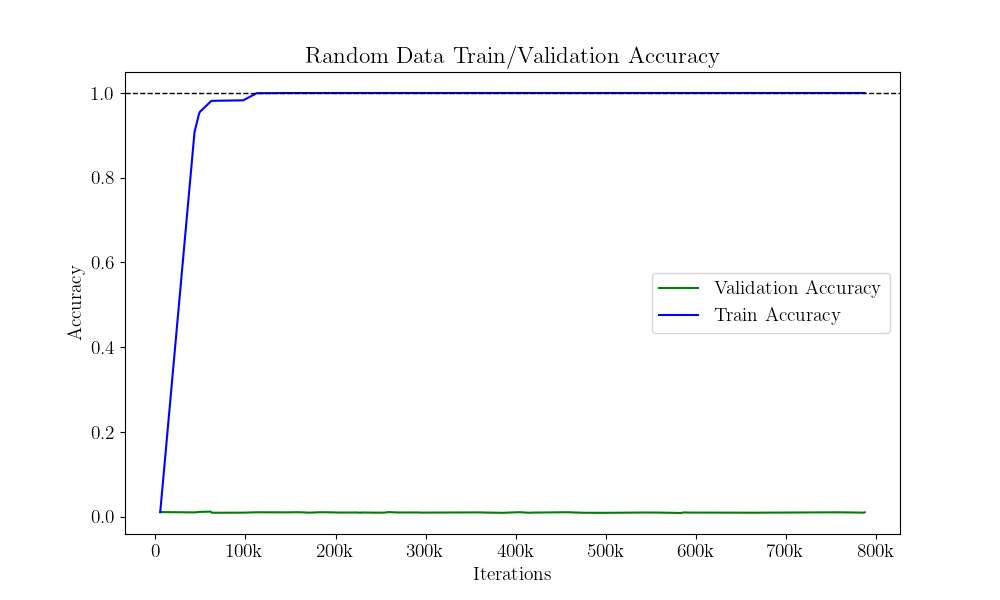
\includegraphics[width=\linewidth,  trim=0 0 0 17mm, clip]{figures/figure_3_1_random_data_run.png}
    \end{subfigure}
    \hfill
    \begin{subfigure}{0.975\linewidth}
        \centering
        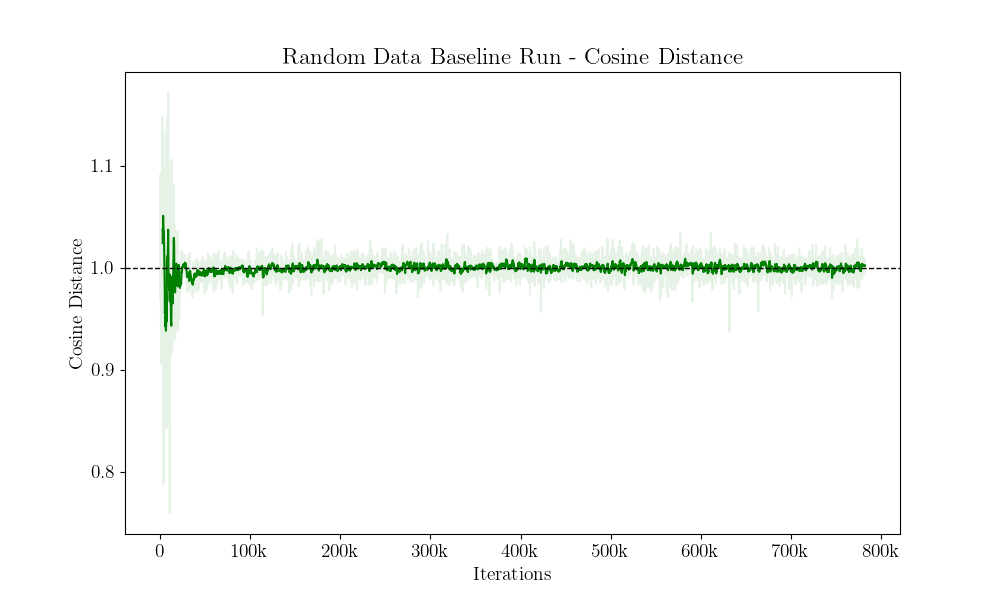
\includegraphics[width=\linewidth,  trim=0 0 0 17mm, clip]{figures/figure_3_2_Random_Data_Run_Cosine_Distance.png}
    \end{subfigure}
   
    \caption{Train and validation accuracy (top) and the cosine distance between micro-gradients (bottom) with rolling average in dark green and raw values in light green, over iterations of a baseline training ResNet18 without GAF on random noise. The model overfits, reaching 100\% training accuracy, but the micro-gradients cosine distance remains above 0.96 throughout the entire training, and above 0.99 for all iterations after the very early iterations. }
    \label{fig:random_data_run}
\end{figure}



With Gradient Agreement Filtering (GAF), instead of blindly averaging all micro-gradients in $\mathcal{M}$, we apply a cosine distance threshold to select only those micro-gradients that are aligned within a given threshold $\tau$, as shown in \Cref{alg:gaf}. Let $\mathbf{g}_i = \nabla_\theta \mathcal{L}(\mathcal{U}_i; \theta)$ denote the micro-gradient for microbatch $\mathcal{U}_i$. The cosine distance between a candidate micro-gradient $\mathbf{g}_i$ and the running sum of accepted gradients $\mathbf{g}$ is $D_c(\mathbf{g}_i, \mathbf{g})$.

We compute a rolling aggregation of micro-gradients starting from the local gradient $\mathbf{g}$ and then checking one by one, and only including those for which $D_c(\mathbf{g}_i, \mathbf{g}) \leq \tau$. We keep a counter $c$ of the agreed upon gradients starting at $c = 1$. Each accepted gradient $\mathbf{g}_i$ is added to the running sum $\mathbf{g}$, and our count $c$ is incremented to keep track of the number of accepted gradients. The filtered macrobatch gradient is
\begin{equation} \label{eq:gaf_grad_update}
   \nabla_\theta \mathcal{L}_{\text{GAF}}(\mathcal{M}; \theta) = \mathbf{g}_{\text{GAF}} = \frac{\mathbf{g}}{c}.
\end{equation}

If no two gradients meet the threshold $\tau$ then $c = 1$ and we skip the update without modifying the optimizer or scheduler as we do not have consensus of any two micro-gradients. Otherwise, the GAF-based SGD update is
\begin{equation}
    \theta \leftarrow \theta - \eta \mathbf{g}_{\text{GAF}}.
\end{equation}

Note, that this implementation is order dependent so could be susceptible to degenerate examples. For example if the initial micro-gradient is orthogonal to all others, then none will agree and the entire macrobatch will be skipped and wasted. This is a shortcoming that could be addressed by tweaking the AllReduce algorithm such that each microgradient acts as the ``initial'' micro-gradient starting from its home GPU, and goes around the ring. The summed micro-gradient with the largest (or smallest) agreement could be the one that is then AllGather'd to the rest of the GPUs. We leave possible implementation to future research. 

% Finally, it is possible to derive that for sufficiently small step size $\eta$, the validation loss and generalization error will be monotonically non-increasing with every GAF step. Such a bound is not possible with standard SGD. If we assume that all samples in the training and validation datasets are sampled i.i.d, and the gradient of our loss function $\nabla_{\theta} \mathcal{L}^{\text{val}}_{\theta}$ is Lipschitz continuous with Lipschitz constants $L \geq 0$, then for a given $\tau$ it is possible to choose an $\eta$ such that our validation loss and generalization error will never increase throughout training. Specifically, if we assume that all samples in the train and validation set are sampled i.i.d, and that the gradient of our loss function  \( \nabla \mathcal{L}^{\text{val}}_{\theta} \) is Lipschitz continuous with Lipschitz constant \( L \geq 0 \), then if we choose a $\tau$ and $\eta$ such that the following inequality always holds: 

% % \[
% % \eta \leq \frac{2 \| g_{\text{batch1}} \| \cos\theta }{L \| g_{\text{batch2}} \| } \leq \frac{2 (1 - \tau) }{L},
% % \]
% \[
% \eta \leq \frac{2 (1 - \tau) }{L},
% \]

% then, every GAF step is guaranteed to maintain or improve validation loss and generalization error. To show how practical this bound is, we empirically estimate L for our architectures to be between 20 and 200. So if we select a $\tau = 0.95$, then if we use a starting $\eta <= 5 \times 10^{-4}$ every step will guarantee a non-increasing validation loss and generalization error. This is exactly what we observe in \Cref{fig:cifarn_does_not_overfit_plot} when we train with $\tau = 0.95$, and set our initial learning rate to $\eta = 5 \times 10^{-4}$. 

% For a complete proof, please see the Appendix. This brings into question whether or not we still need a validation set at all in SGD. 

% With Gradient Agreement Filtering (GAF), instead of blindly averaging all micro-gradients in $\mathcal{M}$, we apply a cosine distance threshold to select only those micro-gradients that are aligned within a given threshold $\tau$ as show in \Cref{alg:gaf}. Let $\mathbf{g}_i = \nabla_\theta \mathcal{L}(\mathcal{U}_i; \theta)$ and $\mathbf{g}_j = \nabla_\theta \mathcal{L}(\mathcal{U}_j; \theta)$ denote the micro-gradients for microbatches $\mathcal{U}_i$ and $\mathcal{U}_j$, respectively. Then, the cosine distance between these micro-gradients is defined by $D_c(\mathbf{g}_i,\mathbf{g}_j)$.

% We compute a rolling aggregation of microgradients sampling one $D_c(\mathbf{g}_i,\mathbf{g}_j) \leq \tau$ with at least one other $\mathcal{U}_i$. The filtered macrobatch gradient is then calculated as
% \begin{equation} \label{eq:gaf_grad_update}
%     \mathbf{g}_{\text{GAF}} = \nabla_\theta \mathcal{L}_{\text{GAF}}(\mathcal{M}; \theta) = \frac{1}{c} \sum_{\mathbf{g} \in \mathcal{G}} \mathbf{g}.
% \end{equation}
% If $|\mathcal{G}|=0$ we just skip the update and do not update our optimizer or scheduler. 

% The GAF-based SGD update is then
% \begin{equation}
%     \theta \leftarrow \theta - \eta \nabla_\theta \mathcal{L}_{\text{GAF}}(\mathcal{M}; \theta).
% \end{equation}

\section{Experiments}
\label{sec:experiments}

To demonstrate the effectiveness of GAF in practice, we train ResNet image classifiers on the CIFAR-100 and CIFAR-100N-Fine datasets using distributed data-parallelism comparing both baseline averaging-based gradient aggregation and GAF-based gradient aggregation. 

\begin{table*}[ht!]
\centering
% \resizebox{\textwidth}{!}{%
\begin{tabular}{@{}lcccccccccc@{}}
\toprule
Dataset & \multicolumn{9}{c}{CIFAR-100} & CIFAR-100N-Fine \\
\midrule
Label Error & 0\% & 5\% & 15\% & 20\% & 30\% & 40\% & 50\% & 60\% & 75\% &  \\
\midrule
GAF & 63\% & 61\% & 60\% & 58\% & 54\% & 53\% & 48\% & 39\% & 13\% & 61.4\%  \\
Averaging & 62\% & 58\% & 53\% & 50\% & 40\% & 38\% & 33\% & 20\% & 11\% & 52.1\% \\
\bottomrule
Improvement & +0.2\% & +3\% & +7\% & +8\% & +14\% & +15\% & +15\% & +19\% & +2\% & +9.3\% \\
\bottomrule
\end{tabular}%
% }
\caption{Image classification validation accuracy of ResNet18 on CIFAR-100 and CIFAR-100N-Fine when trained with GAF-based vs. averaging of micro-gradients. Improvement is the absolute increase in validation accuracy of GAF-based training over the baseline averaging.}
\end{table*}

\subsection{CIFAR-100}

We train RestNet18 on two A40 GPUs on the CIFAR-100 dataset using SGD with momentum and and reduction of the learning rate (learning rate) on validation plateaus with schedule patience of 100 and 0.1 discount. We use an initial learning rate of 0.01. We also applied L2 regularization with a weight decay of 0.01. In all cases, unless otherwise specified, we use a macrobatch of size $m = 200$ with $u = 100$ images per microbatch (exactly 1 sample per class) to ensure each microbatch has the same distribution of data over the training set. We flip each label with a random other classes label for x\% of the labels, for $ x \in \{0,5,15,30,40,50,60,75,80,90\}$, and maintain those incorrect label for the entirety of that run's training (i.e. symmetric noise). For each experiment we found the optimal value of the cosine distance threshold hyperparameter $\tau$ by performing a grid search of values from 0.95 to 1.05 with a step of 0.02 across different batch sizes. We compare with a baseline-training of ResNet18 where the cosine distance threshold is set to 2, which admits all gradients and is equivalent to averaging training weights when $k = 2$. We run for 500k iters for all runs, and observe convergence around 270k iterations for baseline and GAF runs. 

For the no error case, we observe cosine distance threshold of 1 yields best performance. Once errors are introduced we observe a cosine distance of 0.97 provides the best performance. 

As shown in \Cref{fig:cifar100_over_noise_results}, we see a 0.2\% improvement over baseline without added noise to the CIFAR-100 dataset. As we add more and more noise to the labels, the GAF-trained models show increasing improvement over baseline until 60\% where it beats baseline model by 18.4\% when $\tau = 0.97$.

\begin{figure}[t]
    \centering
    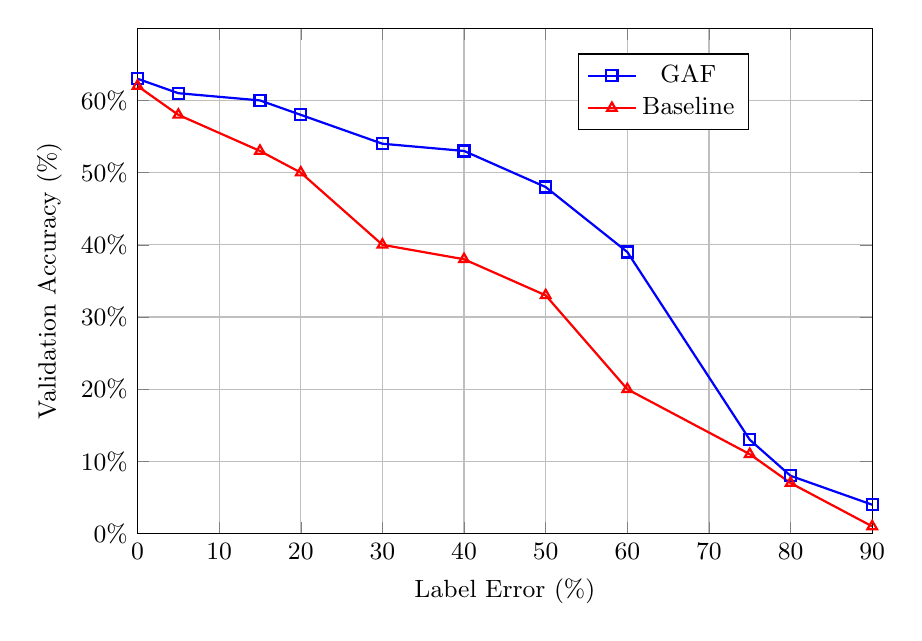
\begin{tikzpicture}
        \begin{axis}[
            width=0.9\linewidth,
            height=8cm,
            xlabel={Label Error (\%)},
            ylabel={Validation Accuracy (\%)},
            xmin=0, xmax=90,
            ymin=0, ymax=70,
            xtick={0, 10, 20, 30, 40, 50, 60, 70, 80, 90},
            ytick={0, 10, 20, 30, 40, 50, 60},
            yticklabel={\pgfmathprintnumber{\tick}\%},
            legend style={font=\small, at={(0.6, 0.95)}, anchor=north west},
            grid=major,
            % title={CIFAR-100 Validation Accuracy of GAF over Baseline},
            label style={font=\small},
            tick label style={font=\small}
        ]

        % Plot for Validation Accuracy - GAF
        \addplot[
            color=blue,
            mark=square,
            thick
        ] coordinates {
            (0, 63) (5, 61) (15, 60) (20, 58) (30, 54) (40, 53) (50, 48) (60, 39) (75, 13) (80, 8) (90, 4)
        };
        \addlegendentry{GAF}

        % Plot for Validation Accuracy - Baseline
        \addplot[
            color=red,
            mark=triangle,
            thick
        ] coordinates {
            (0, 62) (5, 58) (15, 53) (20, 50) (30, 40) (40, 38) (50, 33) (60, 20) (75, 11) (80, 7) (90, 1)
        };
        \addlegendentry{Baseline}

        \end{axis}
    \end{tikzpicture}
    \caption{Validation accuracy on CIFAR-100 with symmetric noisy labels for ResNet18 trained with and without GAF.}
    \label{fig:cifar100_over_noise_results}
\end{figure}

Additionally, we see in \Cref{fig:cifar100_validation_over_cosine_distance} that the performance improvement from GAF-based training ultimately decreases as we increase our cosine distance threshold. As we increase cosine distance threshold beyond 0.97, the improvement from GAF filtering goes away as the filter starts admitting more noise in our gradients, and removing the ability to discern good from bad micro-gradients.

\begin{figure}[ht!]
    \centering
    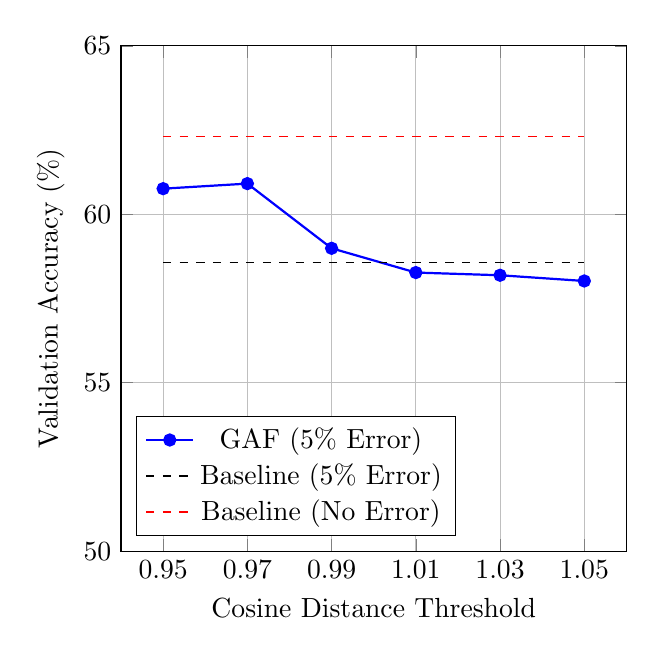
\begin{tikzpicture}
        \begin{axis}[
            % title={GAF over Cosine Distance},
            xlabel={Cosine Distance Threshold},
            ylabel={Validation Accuracy (\%)},
            xmin=0.94, xmax=1.06,
            ymin=50, ymax=65,
            xtick={0.95, 0.97, 0.99, 1.01, 1.03, 1.05},
            ytick={50, 55, 60, 65},
            legend pos=south west,
            grid=both,
            % width=\textwidth,
            width=8cm,
            height=8cm,
        ]

        % Plot validation accuracy
        \addplot[
            color=blue,
            mark=*,
            thick,
        ] coordinates {
            (0.95, 60.76)
            (0.97, 60.91)
            (0.99, 58.99)
            (1.01, 58.27)
            (1.03, 58.19)
            (1.05, 58.02)
        };
        \addlegendentry{GAF (5\% Error)}

        % Lower bound (baseline performance with error)
        \addplot[
            color=black,
            dashed,
        ] coordinates {
            (0.95, 58.57)
            (0.97, 58.57)
            (0.99, 58.57)
            (1.01, 58.57)
            (1.03, 58.57)
            (1.05, 58.57)
        };
        \addlegendentry{Baseline (5\% Error)}

        % Upper bound (baseline performance with no error)
        \addplot[
            color=red,
            dashed,
        ] coordinates {
            (0.95, 62.30)
            (0.97, 62.30)
            (0.99, 62.30)
            (1.01, 62.30)
            (1.03, 62.30)
            (1.05, 62.30)
        };
        \addlegendentry{Baseline (No Error)}

        \end{axis}
    \end{tikzpicture}
    \caption{Validation accuracy of ResNet18 runs trained on CIFAR-100 with GAF over different cosine distance thresholds. As the cosine distance threshold increases beyond 0.97 GAF-based training averages over more noise so generalization decreases. }
     \label{fig:cifar100_validation_over_cosine_distance}
\end{figure}


\subsection{CIFAR-100N-Fine}

To validate GAF on a more realistic noisy dataset, we trained ResNet34 on CIFAR-100N-Fine. CIFAR-100N-Fine is a relabeled version with human annotated noisy labels obtained from one Amazon Mechanical Turk worker, who had a 40.2\% noise rate but in a more structured manner than random as humans are consistently biased in their labels vs. the random flipping done in the CIFAR-100 runs. All CIFAR-100N-Fine training runs use a ResNet34 with PreAct as per the reference paper \cite{wei2022learning}, trained on two A40 GPUs. We additionally test the effect of microbatch size $u$ on the training process by training with and without GAF for batch sizes of $u \in \{100, 200, 300, 400, 500\}$ As with the CIFAR-100 training, we use SGD with momentum and reduce the learning rate on validation plateaus. All other hyper parameters are the same as the CIFAR-100 runs however we do not vary label error percentage since the dataset is already noisy due to the labeling process. The optimal cosine distance threshold parameter $\tau$ is found by varying the value from 0.95 to 1.05 with a step of 0.02. A cosine distance threshold of 2 for the baseline runs, which is equivalent to averaging gradients as it admits all values.

% We run with MVA and static Cosine Distance Thresholding and find that again 0.97 provides the highest value without MVA. 

% ( \textbf{TODO}: Francois include plot)

\Cref{fig:cifarn-microbatch-size} displays the result of these experiments. We find improvement in validation accuracy of training with GAF for all batch sizes, with the largest improvement in validation accuracy of 61.41\% with GAF vs. 52.1\% baseline accuracy for a microbatch size of $u = 100$, which provides a 9.3\% improvement. Note, this is at the smallest microbatch size possible that still contains at least one sample per class (100), while the best performing microbatch size for non-GAF was 200. This means we achieve higher accuracy with half the compute required and could have used half the GPUs (assuming we used multiple processes per GPU). 

Additionally, baseline training on CIFAR-100-N-Fine plateaus at 52.1\% validation accuracy with 100\% train accuracy at 150k iterations. However, even after 600k iterations, GAF-based training surprisingly does not overfit with 59.6\% train accuracy 61.4\% validation accuracy, with slow but continued improvement in both, as shown in \Cref{fig:cifarn_does_not_overfit_plot}.

\begin{figure}[h]
    \centering
    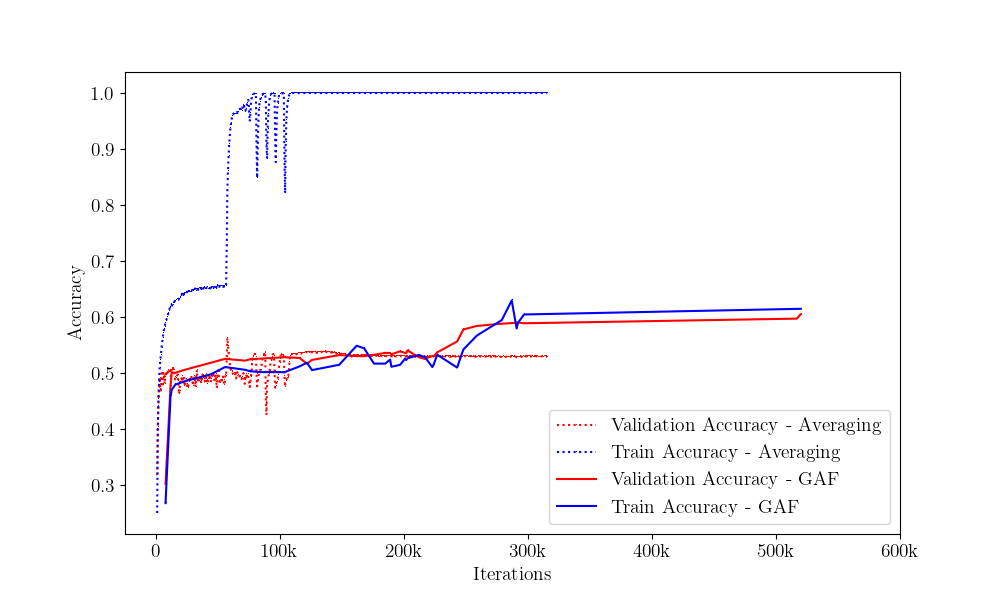
\includegraphics[width=0.975\linewidth]{figures/figure_6_CIFARN_doesnotoverfit_12.png}
    \caption{Train (blue) and validation accuracy (red) over both GAF (solid) and averaging (dotted) runs of ResNet34 of CIFAR-100N-Fine. GAF train accuracy remains very close to validation accuracy, while averaging results in overfitting to the train set within 100k iterations. GAF continues to improve on validation after 500k iterations, albeit very slowly.}
    \label{fig:cifarn_does_not_overfit_plot}
\end{figure}


Finally, we find that the performance improvement from GAF degrades as we increase microbatch size. This means that training can be done with smaller batch sizes and that larger batch sizes in training only increases computational costs without benefit. As with the CIFAR-100 training experiments, the higher we make microbatch size, the benefit of GAF decreases as we begin averaging over more noise and removing the ability for GAF to discern good from bad microbatches. Consequently, we also find that the optimal cosine distance threshold decreases from 0.97 to 0.95 as batch size increases to further increase the filtering as the micro-gradients become increasing correlated. Thus when doing training with GAF following the typical procedure of choosing the largest microbatch size that can fit on a single GPU results in lower validation and instead we should use smaller microbatch sizes and fewer GPUs to achieve higher levels of generalization.

This experiment shows that in addition to a 9.3\% improvement over baseline with a microbatch size of only 100, GAF-based training with smaller microbatches outperforms higher microbatch sizes enabling us to achieve improved training performance with an order of magnitude less compute. 

\begin{figure}[ht!]
    \centering
    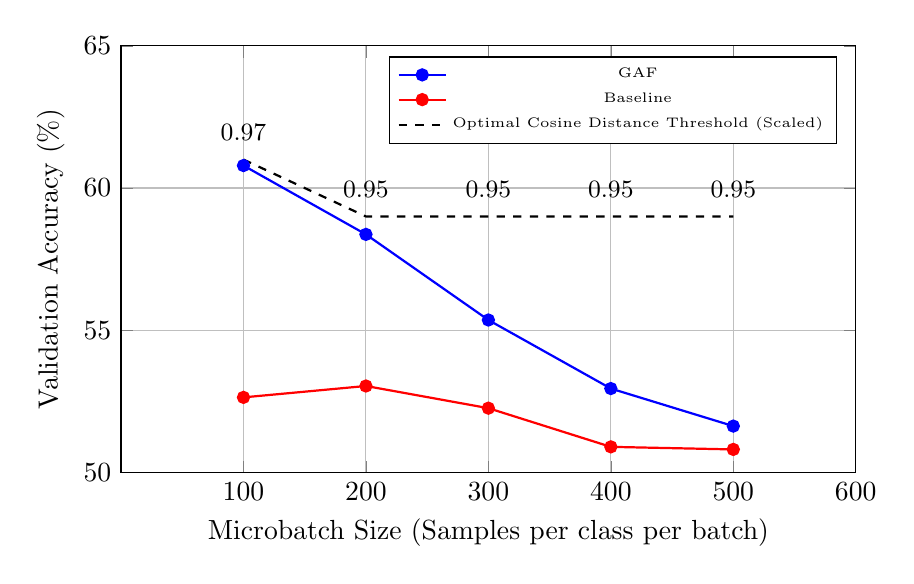
\begin{tikzpicture}
        \begin{axis}[
            % title={Microbatch Size on Validation Accuracy on CIFAR-100N-Fine},
            xlabel={Microbatch Size (Samples per class per batch)},
            ylabel={Validation Accuracy (\%)},
            xmin=0, xmax=600,
            ymin=50, ymax=65,
            xtick={100, 200, 300, 400, 500, 600},
            ytick={50, 55, 60, 65},
            legend style={at={(0.975,0.975)}, anchor=north east, font=\tiny},
            grid=both,
            width=0.9\columnwidth,
            height=7cm,
        ]

        % Plot GAF Validation Accuracy
        \addplot[
            color=blue,
            mark=*,
            thick,
        ] coordinates {
            (100, 60.79)
            (200, 58.37)
            (300, 55.36)
            (400, 52.95)
            (500, 51.63)
        };
        \addlegendentry{GAF}

        % Plot Baseline Validation Accuracy
        \addplot[
            color=red,
            mark=*,
            thick,
        ] coordinates {
            (100, 52.64)
            (200, 53.04)
            (300, 52.26)
            (400, 50.90)
            (500, 50.81)
        };
        \addlegendentry{Baseline}

        % Plot Optimal Cosine Distance Threshold with custom labels
        \addplot[
            color=black,
            dashed,
            mark=none,
            thick,
            nodes near coords={
                \pgfmathparse{\coordindex == 0 ? "0.97" : "0.95"} \pgfmathresult
            },
            every node near coord/.append style={font=\small, anchor=south, yshift=3pt}
        ] coordinates {
            (100, 61) % Approximated y-values to fit within the y-axis range
            (200, 59)
            (300, 59)
            (400, 59)
            (500, 59)
        };
        \addlegendentry{Optimal Cosine Distance Threshold (Scaled)}

        \end{axis}
    \end{tikzpicture}
    
    \caption{ResNet34 PreAct Validation accuracy over microbatch size in the GAF and baseline case on CIFAR-100N-Fine, overlaid with cosine distance threshold used in training. As we increase microbatch size, the benefit of GAF reduces due to averaging more noisy samples.}
    \label{fig:cifarn-microbatch-size}
\end{figure}

% \subsubsection{ImageNet}

% For all ILSVRC12 runs we use ViT-L/16. We train with microbatch size of 380 and a macro batch size of 2. We train on 2xH100s. We use AdamW with a linear warmup of 100 iters and Cosine LR schedule with num cycles = 5 and learning rate 3e-5. We use weight decay of 0.05 and betas of (0.9, and 0.999). As we can not fit one image per class as their are 1000 classes we sample 380 classes of the 1000 and sample 2 images per class and send one to each of the GPU ranks to process so the mini batches are completely iid. We vary cosine distance threshold from 0.95-1.05 with a step of 0.01. We also use cosine distance threshold of 2 for the baseline runs. 

% \subsection{Toy Experiments}
% Omitted for now not working
% \textbf{TODO}: Duncan to fill in.

\section{Conclusions}
\label{sec:conclusions}

In this work, we introduced Gradient Agreement Filtering (GAF) as an alternative to traditional micro-gradient averaging in distributed training. Our experiments on CIFAR-100 and CIFAR-100N-Fine demonstrate the effectiveness of GAF, particularly in scenarios with label noise. By aggregating gradients based on cosine distance, GAF provides a robust approach that improves model performance. Specifically, we observe a 0.2\% improvement on CIFAR-100 without added noise, with progressively larger improvements over baseline training methods as label noise increases, reaching up to an 18.4\% gain at a 60\% noise rate. On the CIFAR-100N-Fine dataset, GAF achieves a 9.3\% improvement over the baseline. We also observe that we are able to maintain the performance improvement even as the microbatch size was reduced, suggesting that we can improve model performance while reducing computational costs.

These results indicate that GAF is a promising approach for improving training stability and accuracy, particularly in noisy environments. The use of cosine distance to filter gradients shows potential not only in mitigating the impact of label noise but also in reducing the computational cost of large-scale distributed training by focusing resources on more aligned gradients.

\section{Future Research Directions}
\label{sec:future_work}

While GAF has demonstrated promising results, several avenues for further research could expand upon its potential and applicability:

\begin{itemize}
    \item \textbf{Alternative Similarity Metrics}: While cosine distance proved effective, other similarity metrics, such as Mahalanobis distance, could be explored to evaluate their impact on GAF’s performance. This could help in tailoring GAF to different types of datasets and noise structures.

    \item \textbf{Adaptive Thresholding}: In this work, we used a fixed cosine distance threshold throughout training. An adaptive threshold that dynamically adjusts based on training progress or model convergence rates may yield improved results, especially in tasks with fluctuating noise levels or diverse data distributions.

    % Commented this one out to hit the page limit of 8 pages
    % \item \textbf{Adaptive Learning Rates}: As we have shown in this paper, disagreement in gradient direction from noisy data signals a lack of confidence in the step. Perhaps it would be appropriate to reduce the step size as a function of the gradient noise across the micro-gradients. For example, if the average micro-gradient cosine distance is small, then we have a lot of confidence in our step and perhaps should increase the step size for this iteration. Alternatively, if the average micro-gradient cosine distance is large, then we have very little confidence in our step and perhaps should decrease the step size for this iteration. 

    \item \textbf{Application to Other Tasks}: GAF was applied to image classification in this study. Extending this technique to other domains, such as natural language processing, speech recognition, or reinforcement learning, could uncover broader benefits and challenges associated with GAF in non-vision tasks. 

    \item \textbf{Memory and Computation Efficiency}: As GAF requires tracking only pairwise cosine distances between micro-gradients, applying this to Ring-AllReduce would be straightforward but would require applying cosine distance to buckets at a time. Ensuring GAF's improvement is maintained despite this is an area of future research, as well as other avenues to optimize compute and memory overhead.
    
    \item \textbf{Order Indifference Techniques}: As GAF is sensitive to the order in which microgradients are processed, perhaps there is a way to augment Ring-AllReduce where during the AllGather phase, the GPU with the highest (or lowest) agreement is the one distributed to all other nodes. 

    \item \textbf{Integration with Advanced Optimizers}: We used standard optimizers like SGD and Adam in our experiments. Investigating how GAF interacts with other advanced optimization techniques, such as Adam, AdamW, LAMB or SHAMPOO, could enhance GAF’s performance, particularly in large-scale or fine-tuning scenarios.

    \item \textbf{Analysis of Gradient Disagreement Dynamics}: Further study of the dynamics of gradient disagreement over the course of training could yield insights into how models converge under noisy conditions and how GAF influences the loss landscape. This might lead to improvements in convergence rates and generalization.

\end{itemize}

Further research in these directions highlight potential improvements and adaptations of GAF, aiming to make it more efficient, robust, and applicable across various deep learning domains. %We hope that our work encourages further exploration of selective gradient aggregation techniques and contributes to advances in distributed deep learning.



% TODO: Uncomment & Write in final version
\documentclass[11pt]{report}
\usepackage[margin=2cm]{geometry}
\usepackage{graphicx}
\usepackage{float}
\usepackage{times}

\begin{document}
\section*{Acknowledgments}
\label{sec:acknowledgments}

\paragraph*{Electricity systems.} We thank James Kelloway (National Grid ESO), Jack Kelly (Open Climate Fix), Zico Kolter (CMU), and Henry Richardson (WattTime) for their help and ideas in shaping this section. We also thank Samuel Buteau (Dalhousie University) and Marc Cormier (Dalhousie University) for their inputs on accelerated science and battery storage technologies; Julian Kates-Harbeck (Harvard) and Melrose Roderick (CMU) for their extensive inputs and ideas on nuclear fusion; and Alasdair Bruce (formerly National Grid ESO) for inputs on emissions factor forecasting and automated dispatch. Finally, we thank Lea Boche (EPRI), Carl Elkin (DeepMind), Jim Gao (DeepMind), Muhammad Hasan (DeepMind), Guannan He (CMU), Jeremy Keen (CMU), Zico Kolter (CMU), Luke Lavin (CMU), Sanam Mirzazad (EPRI), David Pfau (DeepMind), Crystal Qian (DeepMind), Juliet Rothenberg (DeepMind), Sims Witherspoon (DeepMind) and Matt Wytock (Gridmatic, Inc.) for helpful comments and feedback.

\paragraph*{Transportation.}
We are grateful for advice from Alan T.~Jenn (UC Davis) and Prithvi S.~Acharya (CMU) on electric vehicles, Alexandre Jacquillat (CMU) on decarbonizing aviation, Michael Whiston (CMU) on hydrogen fuel cells, Evan Sherwin (CMU) on alternative fuels, and Samuel Buteau (Dalhousie University) on batteries.

\paragraph*{Buildings and Cities.} We thank \'Erika Mata (IVL - Swedish Environmental Research Institute, IPCC Lead Author Buildings section), Duccio Piovani (nam.R) and Jack Kelly (Open Climate Fix) for feedback and ideas.

\paragraph*{Industry.}
We appreciate all the constructive feedback from Angela Acocella (MIT), Kevin McCloskey (Google), and Bill Tubbs (University of British Columbia), and we are grateful to Kipp Bradford (Yale) for his recommendations around embodied energy and refrigeration. Thanks to Allie Schwertner (Rockwell Automation), Greg Kochanski (Google), and Paul Weaver (Abstract) for their suggestions around optimizing industrial processes for low-carbon energy.

\paragraph*{Farms \& Forests.}
We would like to give thanks to David Marvin (Salo) and Remi Charpentier (Tesselo) on remote sensing for land use. Max Nova (SilviaTerra) provided insight on forestry, Mark Crowley (University of British Columbia) on forest fire management, Benjamin Deleener (ChrysaLabs) on precision agriculture, and Lindsay Brin (Element AI) on soil chemistry.

\paragraph{Climate prediction.} We thank Ghaleb Abdulla (LLNL), Ben Kravitz (PNNL) and David John Gagne II (UCAR) for enlightening conversations; Goodwin Gibbins (Imperial College London) and Ben Kravitz (PNNL) for detailed editing and feedback; and Claire Monteleoni (CU Boulder) and Prabhat (LBL) for feedback which improved the quality of this manuscript.

\paragraph*{Societal adaptation.}
We thank Loubna Benabbou (UQAR), Mike Sch{\"a}fer (University of Zurich), Andrea Garcia Tapia (Stevens Tech), Slava Jankin Mikhaylov (Hertie School Berlin), and Sarah M.~Fletcher (MIT) for valuable conversations on the social aspects of climate change. 

\paragraph*{Solar geoengineering.}
We thank David Keith (Harvard), Peter Irvine (Harvard), Zhen Dai (Harvard), Colleen Golja (Harvard), Ross Boczar (UC Berkeley), Jon Proctor (UC Berkeley), Ben Kravitz (Indiana University),  Andrew Lockley (University College London), Trude Storelvmo (University of Oslo), and Simon Gruber (University of Oslo) for help and useful feedback.

\paragraph*{Individual action.} We thank Priyanka deSouza (MIT), Olivier Corradi (Tomorrow), Jack Kelly (Open Climate Fix), Ioana Marinescu (UPenn), and Aven Satre-Meloy (Oxford).

\paragraph*{Collective Decisions.}
We thank Sebastian Sewerin (ETH Z\"urich), D.~Cale Reeves (UT Austin), and Rahul Ladhania (UPenn).

\paragraph*{Education.} We appreciated the constructive feedback received by Jacqueline Bourdeau (T\'{E}LUQ University), who gave us valuable insights regarding the field of AIED.

\paragraph*{Finance.} We thank Himanshu Gupta (ClimateAI), and Bjarne Steffen (ETH Z\"urich) for constructive discussions and the valuable feedback.

\paragraph*{}The authors gratefully acknowledge support from National Science Foundation grant 1803547, the Center for Climate and Energy Decision Making through a cooperative agreement between the National Science Foundation and Carnegie Mellon University (SES-00949710), US Department of Energy contract DE-FG02-97ER25308, the Natural Sciences and Engineering Research Council of Canada, and the MIT Media Lab Consortium.
\end{document}


{
    \small
    %\bibliographystyle{IEEEtranN}
    \bibliographystyle{ieeenat_fullname}
    \bibliography{main}
}

\clearpage 
\appendix 
% \section{Train/Val Loss Bound Proof}
% \label{sec:apppendix_loss_bound_proof}

% Words go here

\end{document}
